% This is "sig-alternate.tex" V2.1 April 2013
% This file should be compiled with V2.5 of "sig-alternate.cls" May 2012
%
% This example file demonstrates the use of the 'sig-alternate.cls'
% V2.5 LaTeX2e document class file. It is for those submitting
% articles to ACM Conference Proceedings WHO DO NOT WISH TO
% STRICTLY ADHERE TO THE SIGS (PUBS-BOARD-ENDORSED) STYLE.
% The 'sig-alternate.cls' file will produce a similar-looking,
% albeit, 'tighter' paper resulting in, invariably, fewer pages.
%
% ----------------------------------------------------------------------------------------------------------------
% This .tex file (and associated .cls V2.5) produces:
%       1) The Permission Statement
%       2) The Conference (location) Info information
%       3) The Copyright Line with ACM data
%       4) NO page numbers
%
% as against the acm_proc_article-sp.cls file which
% DOES NOT produce 1) thru' 3) above.
%
% Using 'sig-alternate.cls' you have control, however, from within
% the source .tex file, over both the CopyrightYear
% (defaulted to 200X) and the ACM Copyright Data
% (defaulted to X-XXXXX-XX-X/XX/XX).
% e.g.
% \CopyrightYear{2007} will cause 2007 to appear in the copyright line.
% \crdata{0-12345-67-8/90/12} will cause 0-12345-67-8/90/12 to appear in the copyright line.
%
% ---------------------------------------------------------------------------------------------------------------
% This .tex source is an example which *does* use
% the .bib file (from which the .bbl file % is produced).
% REMEMBER HOWEVER: After having produced the .bbl file,
% and prior to final submission, you *NEED* to 'insert'
% your .bbl file into your source .tex file so as to provide
% ONE 'self-contained' source file.
%
% ================= IF YOU HAVE QUESTIONS =======================
% Questions regarding the SIGS styles, SIGS policies and
% procedures, Conferences etc. should be sent to
% Adrienne Griscti (griscti@acm.org)
%
% Technical questions _only_ to
% Gerald Murray (murray@hq.acm.org)
% ===============================================================
%
% For tracking purposes - this is V2.0 - May 2012

\documentclass{sig-alternate-05-2015}
% $Id: preamble.tex 456 2014-03-22 21:45:27Z fernando $

\usepackage[draft,inline,noindex,nomargin]{fixme}
\usepackage[english]{babel}
\usepackage{graphicx}
\usepackage{url}
\usepackage{xspace}
\newenvironment{dialogue}%
   {\setlength\topsep{0pt}%
    \begin{small}%
    \begin{it}%
    \begin{list}{}%
         {\setlength{\leftmargin}{.6cm}}%
         \item[]}%
   {\end{list}%
    \end{it}%
    \end{small}} 

\newcommand{\Chatbot}{\textsf{Chatbot}\xspace}
\newcommand{\Alice}{\textsf{Alice}\xspace}
\newcommand{\DA}{\textsf{Dale Aceptar}\xspace}
\newcommand{\Alibi}{``Alibi''\xspace}
\newcommand{\Sect}[1]{Section~\ref{sec:#1}\xspace}
\newcommand{\Tab}[1]{Table~\ref{tab:#1}\xspace}

\newenvironment{tightcenter}{%
  \setlength\topsep{0pt}
  \setlength\parskip{0pt}
  \begin{center}
}{%
  \end{center}
}



\usepackage{minted}
\usepackage{xcolor}
\usepackage{enumitem}
\usepackage{float}
\usepackage{multirow}

% Wraps the figures with a box, and reduces the space above them.
\floatstyle{boxed}
\restylefloat{figure}
\setlength{\intextsep}{10pt}

\newcommand\hs[1]{\mintinline{hs}{#1}}
\newcommand{\faloiDice}[1]{\noindent\textcolor{green}{@faloi: \texttt{#1}}}

\begin{document}

\CopyrightYear{2016} 
\setcopyright{acmcopyright}
\conferenceinfo{ITiCSE '16,}{July 09-13, 2016, Arequipa, Peru}
\isbn{978-1-4503-4231-5/16/07}\acmPrice{\$15.00}
\doi{http://dx.doi.org/10.1145/2899415.2899460}

% Copyright
%\setcopyright{acmcopyright}
%\setcopyright{acmlicensed}
%\setcopyright{rightsretained}
%\setcopyright{usgov}
%\setcopyright{usgovmixed}
%\setcopyright{cagov}
%\setcopyright{cagovmixed}


% DOI
%\doi{10.475/123_4}

% ISBN
%\isbn{123-4567-24-567/08/06}

%Conference
%\conferenceinfo{PLDI '13}{June 16--19, 2013, Seattle, WA, USA}

%\acmPrice{\$15.00}

%
% --- Author Metadata here ---
%\conferenceinfo{WOODSTOCK}{'97 El Paso, Texas USA}
%\CopyrightYear{2007} % Allows default copyright year (20XX) to be over-ridden - IF NEED BE.
%\crdata{0-12345-67-8/90/01}  % Allows default copyright data (0-89791-88-6/97/05) to be over-ridden - IF NEED BE.
% --- End of Author Metadata ---

\title{A comparison of CS1 and CS3 students learning \\ functional programming using an online coding tool}
%\subtitle{[Extended Abstract]
%\titlenote{A full version of this paper is available as
%\textit{Author's Guide to Preparing ACM SIG Proceedings Using
%\LaTeX$2_\epsilon$\ and BibTeX} at
%\texttt{www.acm.org/eaddress.htm}}}
%
% You need the command \numberofauthors to handle the 'placement
% and alignment' of the authors beneath the title.
%
% For aesthetic reasons, we recommend 'three authors at a time'
% i.e. three 'name/affiliation blocks' be placed beneath the title.
%
% NOTE: You are NOT restricted in how many 'rows' of
% "name/affiliations" may appear. We just ask that you restrict
% the number of 'columns' to three.
%
% Because of the available 'opening page real-estate'
% we ask you to refrain from putting more than six authors
% (two rows with three columns) beneath the article title.
% More than six makes the first-page appear very cluttered indeed.
%
% Use the \alignauthor commands to handle the names
% and affiliations for an 'aesthetic maximum' of six authors.
% Add names, affiliations, addresses for
% the seventh etc. author(s) as the argument for the
% \additionalauthors command.
% These 'additional authors' will be output/set for you
% without further effort on your part as the last section in
% the body of your article BEFORE References or any Appendices.

%\numberofauthors{8} %  in this sample file, there are a *total*
% of EIGHT authors. SIX appear on the 'first-page' (for formatting
% reasons) and the remaining two appear in the \additionalauthors section.
%
\numberofauthors{4}
\author{
% % You can go ahead and credit any number of authors here,
% % e.g. one 'row of three' or two rows (consisting of one row of three
% % and a second row of one, two or three).
% %
% % The command \alignauthor (no curly braces needed) should
% % precede each author name, affiliation/snail-mail address and
% % e-mail address. Additionally, tag each line of
% % affiliation/address with \affaddr, and tag the
% % e-mail address with \email.
% %
 % 1st. author
 \alignauthor
% Luciana Benotti\\
%       \affaddr{LIIS Group, FaMAF}\\
%       \affaddr{Universidad Nacional de C\'ordoba/CONICET}\\
       %%\affaddr{Ciudad Universitaria, 
%		   \affaddr{C\'ordoba, Argentina}\\
%        \email{luciana.benotti@unc.edu.ar}\\
 % 2nd. author
 \alignauthor
% Federico Aloi\\
%        \affaddr{Mumuki Project}\\
%        \affaddr{Buenos Aires}\\
%				\affaddr{Argentina}\\
%        \email{fede@mumuki.org}\\
 % 3rd. author
 \alignauthor 
% Franco Bulgarelli\\
%         \affaddr{Mumuki Project}\\
%        \affaddr{Buenos Aires}\\
%				\affaddr{Argentina}\\
%        \email{franco@mumuki.org}\\ \and  % use '\and' if you need 'another row' of author names
 %% 4th. author
\alignauthor Marcos J. G\'omez\\
\affaddr{LIIS Group, FaMAF}\\
       \affaddr{Universidad Nacional de C\'ordoba}\\
       %%\affaddr{Ciudad Universitaria, 
		   \affaddr{C\'ordoba, Argentina}\\
       \email{mgomez4@famaf.unc.edu.ar}		
% % 5th. author
\alignauthor Guillaume Hoffmann\\
\affaddr{LIIS Group, FaMAF}\\
       \affaddr{Universidad Nacional de C\'ordoba/CONICET}\\
       %%\affaddr{Ciudad Universitaria, 
		   \affaddr{C\'ordoba, Argentina}\\
       \email{guillaume.hoffmann@conicet.gov.ar}	
% \alignauthor Sean Fogarty\\
%        \affaddr{NASA Ames Research Center}\\
%        \affaddr{Moffett Field}\\
%        \affaddr{California 94035}\\
%        \email{fogartys@amesres.org}
% % 6th. author
% \alignauthor Charles Palmer\\
%        \affaddr{Palmer Research Laboratories}\\
%        \affaddr{8600 Datapoint Drive}\\
%        \affaddr{San Antonio, Texas 78229}\\
%        \email{cpalmer@prl.com}
 }
% % There's nothing stopping you putting the seventh, eighth, etc.
% % author on the opening page (as the 'third row') but we ask,
% % for aesthetic reasons that you place these 'additional authors'
% % in the \additional authors block, viz.
% \additionalauthors{Additional authors: John Smith (The Th{\o}rv{\"a}ld Group,
% email: {\texttt{jsmith@affiliation.org}}) and Julius P.~Kumquat
% (The Kumquat Consortium, email: {\texttt{jpkumquat@consortium.net}}).}
% \date{30 July 1999}
% % Just remember to make sure that the TOTAL number of authors
% % is the number that will appear on the first page PLUS the
% % number that will appear in the \additionalauthors section.

\maketitle
\begin{abstract}
This paper describes an observational study in two different universities on courses teaching Haskell in CS1 and CS3 of Computer Science degrees in Argentina. In these courses a web-based coding tool that provides automatic formative feedback and assessment was used to teach fundamental functional programming concepts and constructs to 17-30 year old students. We analyse students' performance and learning process based on programming exercises, tests, questionnaires and system logs. Data shows that the use of the automated assessment tool seems to decrease course dropouts particularly in CS1. %The tool promotes student spontaneous exploration of other programming languages. These findings imply that ...
\end{abstract}


%\begin{CCSXML}
%<ccs2012>
%<concept>
%<concept_id>10003456.10003457.10003527.10003541</concept_id>
%<concept_desc>Social and professional topics~K-12 %education</concept_desc>
%<concept_significance>500</concept_significance>
%</concept>
%</ccs2012>
%\end{CCSXML}

\ccsdesc[500]{Language Classifications~Applicative (functional) languages}
\ccsdesc[500]{Computers and Education~Computer-assisted instruction}

%
%  Use this command to print the description
%
%
\printccsdesc

% We no longer use \terms command
%\terms{Theory}

\keywords{Functional programming; Haskell; Coding tools; Replication; Automatic assessment}
\section{Introduction} \label{introduction} 

%length: 1 page including headings
%resposible: Lu & Gui

%content:
%introduction and motivation

No matter what programming language students are learning they need a lot of practice in order to get good at it. Also, the practice is more effective if it is guided by useful formative feedback. However, teacher feedback is costly and slow. As a result, there are many coding tools that offer programming exercises and provide automated feedback
on student solutions. According to a recent review~\cite{Keuning:2016}, most of these tools support imperative programming languages and less than 10\% of them support functional programming. 

Many coding tools not only generate automated formative feedback, but they also log large amounts of educational data. As argued by previous work~\cite{Ihantola:2015}, these logs could feed educational data mining in order to better understand student behaviour. However, the majority of the studies are conducted within a single institution and a single course lowering the reliability of the results.

The goal of this paper is to investigate how students with different backgrounds use an online coding tool and how this influences their behaviour when learning functional programming. We designed an observational study to compare how CS1 students (with no previous background in programming), and CS3 students (with two previous semesters of imperative programming courses) use an online coding tool to learn Haskell. We piloted CS lessons in two different universities. Our courses focused on modularity and function composition, conditionals, pattern matching, lists, tuples, and recursion. %We analysed student behaviour while using a web-based coding tool and compared male and female performance. 
The main contributions of this paper are:
\begin{itemize}
\setlength\itemsep{0pt}
\setlength{\parskip}{0pt}
\item Analyse how students with different background learn a functional programming language. 
\item Introduce a web-based coding tool that generates automated formative feedback for Haskell 
\item Evaluate gender and background differences in indicators of learning and engagement in CS1 and CS3. 
\end{itemize}

We begin the paper by describing the online coding tool for Haskell that we use, called Mumuki, and its rationale. Then, we address the study design followed by our findings. We analyse student performance discriminated by their background and gender. Moreover, we discuss common errors in students learning functional programming in our courses. Finally, we summarise previous work on educative coding tools to teach functional programming. We close this paper with conclusions and implications for teaching Haskell at different university levels.



%list of contributions of the paper
%plan of the paper





 %1 page (Lu) including title, abstract


\section{Mumuki: An online coding tool} \label{the-approach}

%length: 1 page
%resposible: Fede & Franco

%content:
%general descrition of Mumuki
%description and example of test cases and expectations

Mumuki is a free and open source\footnote{Source code available at \url{https://github.com/mumuki}.} web-based coding tool that provides automatic formative feedback and assessment, developed in Argentina. This platform provides assistance for teachers and students, in a process conducted by practice where theory arises from the exercises. It supports several programming languages: Haskell, Prolog, Python, JavaScript and C. Mumuki is currently used at six Argentinian universities, five high schools and two coding clubs\footnote{The complete list of organizations using Mumuki can be found at \url{http://www.mumuki.org} (in Spanish).}, with more than 1500 active users.

Practice within the platform is organised across topics with many programming exercises\footnote{The exercises are available at \url{http://mumuki.io}} each. An exercise includes two 
parts. On the one hand, it includes a description of the problem the student should solve by providing a program, in which generally, no more than a few functions are required. On the other hand, the exercise designer provides a way to automatically compute feedback for the solution of the exercise at two different levels: correctness and quality. For correctness, a suite of representative unit tests are provided by the teacher and executed against the final program. The final program could include auxiliary functions  programmed by the teacher. Although correctness cannot be assured by this technique, it proved to be good enough for the complexity  of the existent exercises. Regarding the quality of the student solution, the abstract syntax tree is used. By using an editor tool, the teacher can pick several predefined patterns, called \emph{expectations} in Mumuki. Expectations are defined so that
they must be present or not present in the student’s solution. When the student submits a solution, each expectation is evaluated against it.

%The teacher defines a set of regular expressions, called \emph{expectations} in Mumuki, specifying patterns that should be present in the student's solution. When the student submits a solution, each expectation is evaluated against it.

Imagine the following scenario. When explaining lists, the teacher wants to write an exercise to introduce the \hs{filter} function. This exercise asks the student to define a function called \hs{onlyEvenNumbers} that returns only the even numbers of a given list. The exercise description is illustrated by the example \hs{onlyEvenNumbers [8,7,6,5] = [8,6]}. 
The following unit tests are provided by the exercise designer and not shown to the student until he submits a solution.
\begin{itemize}[noitemsep,topsep=0pt]
    \item {Expect \hs{onlyEvenNumbers [] = []}.}
    \item {Expect \hs{onlyEvenNumbers [1,2,3] = [2]}.}
    \item {Expect \hs{onlyEvenNumbers [7,14,9,10] = [14,10]}.}
\end{itemize}

The teacher also defines the following expectations. Because the use of \hs{filter} is expected, direct recursion is not allowed. This is specified by the teacher as a pattern that \emph{should not} be found in the student solution. Also, the teacher wants to encourage code reuse, so the solution must use the \hs{even} function provided by Haskell's standard libraries. This is specified by the teacher as a pattern that \emph{should} be found in the student solution. 
%Summing up, the exercise expectations are the following.
%\begin{itemize}[noitemsep,topsep=0pt]
%    \item {\hs{onlyEvenNumbers} should not use direct recursion.}
%    \item {\hs{onlyEvenNumbers} should use \hs{even}.}
%\end{itemize}

In Figure~\ref{fig:recursion} the student uses \hs{even} but she uses direct recursion instead of using \hs{filter} in the solution. Mumuki informs the test results are correct but an expectation is not met. It explains that the student must not use recursion. The exercise is assessed by Mumuki as yellow: tests results are correct but some expectation is not met. 

In Figure~\ref{fig:error} the student did not use \hs{even} and he made a mistake when programming his version of even. Instead of verifying that the modulus operation is zero, he compares it to one. Both the tests and one of the expectations fail, and this is reported by Mumuki. The exercise is assessed by Mumuki as red because some test results are incorrect. 

\begin{figure}

%\textbf{Solution:}
\begin{minted}{haskell}
SOLUTION: onlyEvenNumbers [] = []
          onlyEvenNumbers (x:xs)
            | even x    = x:(onlyEvenNumbers xs)
            | otherwise = onlyEvenNumbers xs

FEEDBACK:
\end{minted}
%\textbf{Feedback:}\\
%\ \\
\vspace*{-0.7cm}
\hspace*{1.5cm}\mbox{
    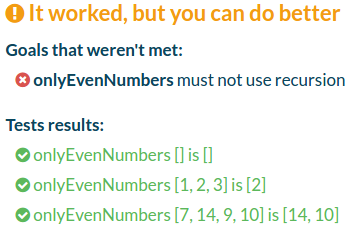
\includegraphics[width=0.32\textwidth]{screenshots/atheneum-warning-direct-recursion-used.png}
    }
    
\caption{Sample solution to an exercise which is assessed as yellow by Mumuki because test results are correct but some expectation is not met.\label{fig:recursion}}

\end{figure}    

Student solutions are assessed by Mumuki with three possible values: red, yellow or green. Red indicates that some test result is not correct. Yellow means that all tests are correct but some expectation is not met. An exercise is marked green when all tests are correct and all expectations are met. 

Every solution submitted by a student is stored, thus the teacher has access not only to the final solution but also to all the steps that lead to it. The timestamp, the tests and expectations results, the result of the execution and the status that was reported to the student are also stored, so the full history can be reproduced. This information, along with the student's profile, could be useful to improve the exercises, to explore common mistakes, etc.

\begin{figure}[H]
%\textbf{Solution:}
\begin{minted}{haskell}
SOLUTION: onlyEvenNumbers ls = 
            filter (\x -> x `mod` 2 == 1) ls

FEEDBACK:
\end{minted}
    
%\textbf{Feedback:}\\
%\ \\
\vspace*{-0.7cm}
\hspace*{1.5cm}\mbox{
    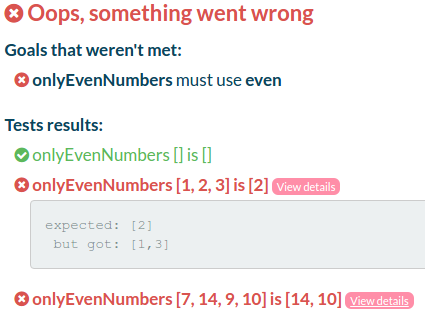
\includegraphics[width=0.4\textwidth]{screenshots/atheneum-error-tests-failed.png}
}
    
    \caption{Sample solution to an exercise that is assessed as red by Mumuki because some tests results are incorrect.\label{fig:error}}
\end{figure} 

The logged data is presented on a web page as shown in Figure~\ref{fig:classroom} and can be accessed only by the teachers. In the web interface, the teachers can monitor students' progress, view the difference between submissions and send comments to the student about particular solutions. 

Two solutions for the same exercise and their difference are reported on the teacher's tool, using a diff highlighting library that allows to visualise it in either way. Visualisation can be \emph{unified} showing line by line differences in the same panel and highlighting the differences as illustrated in Figure~\ref{fig:classroom}. Or it can be \emph{split} side by side, with two different panels showing two different submitted solutions. The figure also shows the textbox that the teacher can  use to send comments associated to a particular student submission. In the figure, the student has submitted ten different solutions for this exercise. The last one is marked green by Mumuki since it passes all the tests and meets all the expectations. 

\begin{figure}
    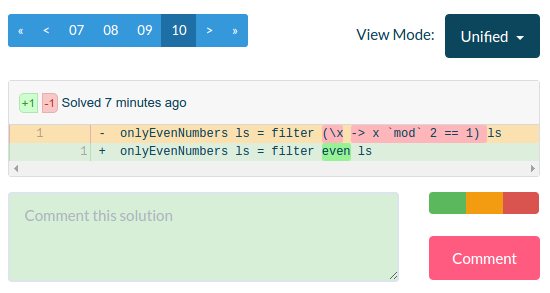
\includegraphics[width=0.46\textwidth]{screenshots/classroom-unified-diff.png}
    
    \caption{Two solutions for the same exercise and their difference are reported on the teacher's tool, using a diff highlighting tool.}
    \label{fig:classroom}
\end{figure}
 %1 page (Fede & Franco), mumuki description

\section{Study Design} \label{study-design}

%length: 1 page
%responsible: Lu & Gui

%content:
%sample demographics
%description of the data collection
%description of the data analysis
%describe groups of students, demographics, define objective and automatic metrics, subjective and self reported, TAM

We describe the contexts where we conducted the observational study outlining the different interventions performed and the data that was collected. 

\subsection{Data Collection and Analysis}

We performed interventions in two different public universities. In both of them we taught Haskell using Mumuki. %In particular we taught function composition, modularity and parameters, types, conditionals and pattern matching, lists and tuples and direct recursion.  

Most previous work reporting learning experiences using an educative coding tool are conducted within a single institution and a single course. We selected two institutions that introduce functional programming with Haskell but have groups of students with different characteristics to replicate our observational study and validate our results. One of the public universities, called UTN, introduces Haskell to CS3 students while the other, called UNC introduces Haskell to CS1 students. In total, 114 students participated in this observational study. 59 students at CS3 level and 55 students at CS1 level.

%\subsection{Data Collection and Analysis}

%\begin{table}[h]
%\begin{small}
%\begin{tabular}{|l|c|c|c|c|}
%\hline
%University level 					           & HS & CS1 & CS3 & CS8    \\
%\hline
%Number of students at the start & 7  & 55 & 59   & 8 \\
%\hline
%Number of students at the end & 7  & 36 & 51   & 6 \\
%\hline
%\end{tabular}
%\end{small}
%\caption{Participants Distribution. The difference between the number of student at the start and end of the course indicates course dropouts.
%}
%\label{table:part_dist}
%\end{table}

%In the following subsections we describe the universities contexts where we conducted the observational study outlining the different interventions in CS1 and CS3. In Section~\ref{findings} we report the quantitative and the qualitative results. 

All students programmed in Haskell employing concepts such as function composition and modularisation, conditional control structures, pattern matching, list structures and functions on lists, and recursion as a fundamental repetition control structure. The students in both groups had to solve the same Haskell exercises in Mumuki. Students were asked to solve 82 programming exercises divided in five topics. Using the same exercises allowed for comparison of the students understanding in the two groups.

%All the students were evaluated with a final test that evaluated the taught concepts. The difference between the number of student participating and tested indicates course dropouts.

We asked the students to complete a questionnaire designed following the Technology Acceptance Model (TAM) methodology~\cite{Chuttur:2009} in order to evaluate their attitude towards Mumuki. 

We also conducted lesson observations during the Haskell programming classes. Observations allowed us to gather data on student understanding, engagement and on transferring concepts learnt with other languages. In this paper, we only report on the Haskell programming stage to compare how students with different programming background learnt basic programming concepts and applied them to functional programming. We do not present data on students learning other programming languages. 

After the course all the students were evaluated with a written  exam. Neither Mumuki nor other compiler was used for the exam. The exam was manually corrected by the teachers.

Because the focus of this paper is understanding how different background group of students learn functional programming, we compared results of the different interventions. In the next section we show exercise results with descriptive statistics. We crossed CS1 and CS3 data and compared gender differences. We triangulated these results with qualitative data from observations that provided further indicators of emerging themes. 

\subsection{The CS1 Intervention}

From August to October 2016 a university professor, two teaching assistants and one student assistant taught 15 four-hour functional programming lessons to CS1 students at UNC. The course was taught for eight hours a week divided in two days from 9am to 1pm. This is the first programming course of a 5-year degree in Computer Science. The course started with 55 students that enrolled and attended the course at least two days. From the 55 students, only 2 reported previous experience programming with imperative languages and none of them reported experience with functional programming. The average age was 21 years old. Each 4-four hour lecture was divided in two stages of two hours each. 

During the first stage, the students used Mumuki in the laboratory programming functions in Haskell. Mumuki provided automated formative feedback but also the professor and the teaching assistants walked around the laboratory answering questions about the exercises. 

During the second stage, the students went to a classroom  where the professor explained in the blackboard the concepts practised in the laboratory, presented worked out examples and discussed the most commonly observed errors. No computer was used in the classroom. Students were encouraged to program in Haskell using paper and pencil and to propose test cases in order to manually evaluate their programs. 

Summing up, during the course, students used Mumuki during 30 hours. They also used Mumuki outside the course but 80\% of their submissions were made during class hours. 

\subsection{The CS3 Intervention}

From March to May 2016 a university professor, two teaching assistants and six student assistants taught 9 four-hour functional programming lessons to CS3 students at UTN. The course was taught for four hours a week in a single day from 9am to 1pm. Before this course, all the students learn imperative programming in Pascal and C during two semesters. The course started with 59 students that attended the course for at least two classes. In the previous  semesters, Pascal and C languages were used to teach classical control structures and basic data structures such as lists, stacks, and queues. None of the students reported previous experience with functional programming. The average age was 22 years old.

During the classes, Mumuki was used to introduce new concepts and to practice previously learnt ones. When considered necessary by the professor or the teaching assistant, they stopped the practice and explained some concept in the blackboard or screen projector using Mumuki, discussing errors and sharing different solutions. These explanations lasted 10 minutes in average and never took more than 10\% of the total time. Students were not asked to program on paper and they used Mumuki during the whole lecture. 

Summing up, during the course, students used Mumuki during 36 hours. They also used Mumuki outside the course, 70\% of their submissions were made during class hours.  %1 page (Lu, Gui, Franco), describe groups of students, demographics, define objective and automatic metrics, subjective and self reported, TAM

\section{Findings} \label{findings}
%length: 1 page
%resposible: everybody
%content:

In this section we describe our comparative findings in CS1 and CS3. We start by describing the dropout rates and pass rates in CS1 and CS3. Then we describe the student  performance on the exercised offered in Mumuki per topic. Finally we present our results of applying the Technology Acceptance Model (TAM) to evaluate the acceptance of Mumuki as a tool for supporting learning of Haskell. 

\subsection{Dropout and pass rates}

Tables~\ref{utnCS3} and~\ref{uncCS1} show the dropout and pass rates in CS3 and CS1 during the years 2014, 2015 and 2016. Mumuki was only used during 2016. During 2014 and 2015 the students used directly a compiler (Hugs or Ghci) in order to solve the programming exercises.  

\begin{table}
\begin{tightcenter}
\setlength\tabcolsep{1.9pt}
\begin{tabular}{|l|c|c|c|c|c|c|c|c|c|c|c|c|c|c|c|}

\hline
    & \multicolumn{5}{ |c| }{2014}       
    & \multicolumn{5}{ |c| }{2015}       
    & \multicolumn{5}{ |c| }{2016} \\

\hline
    & S & D & P   & \emph{\%D} & \emph{\%P}  
    & S & D & P   & \emph{\%D} & \emph{\%P} 
    & S & D & P   & \emph{\%D} & \emph{\%P} \\
    
\hline
F	    
    & 7     & 3  & 3   & \emph{43} & \emph{43}	 
    & 6     & 0  & 3   & \emph{0}  & \emph{50}
    & 13    & 1  & 4   & \emph{8}  & \emph{31} \\

\hline    
M	    
    & 44    & 10 & 16   & \emph{23} & \emph{36} 
    & 40	& 13 & 12   & \emph{33} & \emph{30}  
    & 46    & 7  & 18   & \emph{15} & \emph{39} \\
    
\hline
n	    
    & 51    & 13  & 19 & \emph{\textbf{25}} & \emph{\textbf{37}}  
    & 46	& 13  & 15 & \emph{\textbf{28}} & \emph{\textbf{33}} 
    & 59    & 8   & 22 & \emph{\textbf{14*}} & \emph{\textbf{37}} \\

\hline
\end{tabular}
\end{tightcenter}
\caption{Dropout (\%D) and passed rates (\%P) in CS3 at UTN in 2014, 2015 and 2016 discriminated by gender. S stands for Started the course, f for female and m for male. Significant differences are marked with *.}
\label{utnCS3}
\end{table}

Table~\ref{utnCS3} shows that use of Mumuki seems not to have an impact on the pass rate. The pass rate in 2016 is 37\% which is not significantly different of the rates in 2015 (33\%) and 2014 (37\%). We performed a Pearson correlation analysis of each student performance in Mumuki versus his mark in the final test and no correlation was found. However, a significant decrease in the dropout rate can be observed the year Mumuki was used. The dropout rate in 2016 is 14\% while it was 28\% and 25\% in the previous years.  

\begin{table}
\begin{tightcenter}
\setlength\tabcolsep{1.9pt}
\begin{tabular}{|l|c|c|c|c|c|c|c|c|c|c|c|c|c|c|c|}

\hline
    & \multicolumn{5}{ |c| }{2014}       
    & \multicolumn{5}{ |c| }{2015}       
    & \multicolumn{5}{ |c| }{2016} \\

\hline
    & S & D & P   & \emph{\%D} & \emph{\%P}  
    & S & D & P   & \emph{\%D} & \emph{\%P} 
    & S & D & P   & \emph{\%D} & \emph{\%P} \\
    
\hline
F	    
    & 12    & 9  &  2   & \emph{75}  & \emph{17}	 
    & 17    & 10 &  4  & \emph{59}  & \emph{24}
    & 12    & 3  &  7  & \emph{25}  & \emph{58} \\

\hline    
M	    
    & 54    & 29 & 19   & \emph{54} & \emph{35} 
    & 41	& 24 & 14   & \emph{59} & \emph{34}  
    & 43    & 16 & 14   & \emph{37} & \emph{33} \\
    
\hline
n	    
    & 66    & 38  & 21 & \emph{\textbf{58}} & \emph{\textbf{32}}  
    & 58    & 34  & 18 & \emph{\textbf{59}} & \emph{\textbf{31}} 
    & 55    & 19  & 21 & \emph{\textbf{35*}} & \emph{\textbf{38}} \\
    
%\hline
%\emph{\%Female} 
%    & \emph{22\%}   & \emph{23\%}   &   
%    & \emph{13\%}	& \emph{18\%}   &   
%    & \emph{14\%}   & \emph{10\%}   &  \\

\hline
\end{tabular}
\end{tightcenter}
\caption{Dropout (\%D) and passed rates (\%P) in CS1 at UNC in 2014, 2015 and 2016 discriminated by gender. S stands for Started the course, f for female and m for male. Significant differences are marked with *.}
\label{uncCS1}
\end{table}

Table~\ref{uncCS1} shows dropout and passed rates for the CS1 students at UNC. Again Mumuki does not have an impact on the pass rate and no correlation is found between student performance in Mumuki and their mark in the exam. However, an important decrease in dropout rate can be observed the year Mumuki was used. The dropout rate in 2016 is 38\% while it was 59\% and 58\% in the previous years.  

These results are consistent with previous work~\cite{Kumar:2008} on imperative and object oriented languages. Kumar claims that online coding tools similar to Mumuki can be used to improve the retention of students in Computer Science. This is particularly useful in the first CS courses when student's self-confidence is lower. Kumar also claims that the impact is stronger on female students. Our results are not conclusive in this respect probably because of the small percentage of female students. 

The dropout rate in our observational study is high when comparing it to the one in other countries reported in previous work with an
average of 15\% ~\cite{Watson:2014}. Probable causes could be among the following. Both UNC and UTN are public universities and hence they are completely free. Some students work during their studies and others have weak backgrounds in mathematics and need more time to catch up. In general, students that dropout in CS1 quit studying CS. However, students that do not dropout and fail the exam (considered in
the tables) get multiple chances to take it again.    

\subsection{Performance per topic}

We  analyse  student  performance on the different programming topics covered in our course  discriminated  by course level.   Moreover,  we  discuss  common errors in students learning functional programming in our courses. 

We extracted this information automatically from the the system logs. They contain almost 20000 submissions for CS1 with an average of approximately 8 submissions per exercise per student. They contain almost 16000 submissions for CS3 with an average of approximately 5 submissions per exercise per student.  

Figure~\ref{fig:success-rate-by-course} summarises the results of the exercises that the students completed in Mumuki. It indicates the average percentage of exercises assessed in green by Mumuki. The results are presented discriminated by background (CS1 vs CS3). The topics are function composition (including modularity, parameters and simple types), conditionals and boolean operators, pattern matching and tuples, lists and recursion as a basic iterative control structure. 

From the figure we can observe that the CS1 students performance decreases when they start with pattern matching. Observing Mumuki logs and the lecture observations we see one frequent error in this topic. Students do not realise that the order in which they write the patterns may matter. Take for instance the following example. 

\begin{figure}
    \centering
    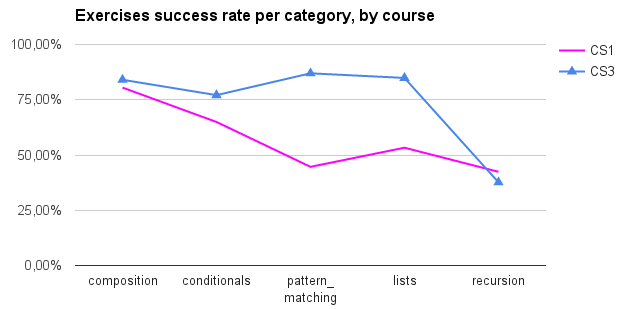
\includegraphics[width=0.4\textwidth]{graphics/success-rate-per-category-by-course.png}
    \caption{Percentage of green exercises per CS group and topic. The topics include function composition, conditionals, pattern matching, lists and recursion.}
    \label{fig:success-rate-by-course}
\end{figure}

\begin{minted}{haskell}
  count0 :: (Show a) => (Int,Int) -> String
  count0 (x,y) = "The pair contains no zero"
  count0 (x,0) = "The pair contains one zero"
  count0 (0,y) = "The pair contains one zero"
  count0 (0,0) = "The pair contains two zeros"
\end{minted}

The last three lines of this program will never be used and the function will always return "The pair contains no zero" even when it contains a zero. This is because all pairs match the pattern (x,y). However, if the order of the lines is inversed the program will work correctly. This error is not common in CS3 probably because of the students' previous experience with imperative programming.

The performance in CS3 decreases in the last topic: recursion. It could be argued that recursion is the control structure that differs the most to the ones learned in imperative programming. A common error is to enter an infinite loop as illustrated in the following example.  

\begin{minted}{haskell}
  delete :: a -> [a] -> [a]
  delete n [] = []
  delete n (x:xs) | n == x = delete n xs
                  | otherwise = delete n (x:xs)
\end{minted}


\subsection{Usefulness and ease of use}

Finally we analyse whether CS1 and CS3 students perceive the usefulness and ease of use differently. To this goal we applied the Technology Acceptance Model (TAM)~\cite{Chuttur:2009}. We performed a survey to all the students that did not dropout (n=87). We asked the students to indicate their level of agreement with the statements listed in Table~\ref{tam-ease-of-use} using a 7-point Likert scale (from 1 to 7). We also asked students to provide free text comments on the best and the worst features of Mumuki.  

CS3 students rate Mumuki less positively in most questions regarding usefulness (statements 1 to 6). The difference in statement 4 is significant (0.99). CS3 students average value for ``Mumuki offers help when I find a task difficult'' is 4.53. 
%The automatic feedback generated by Mumuki includes the results 
%of the test cases and expectations and the output of the compiler. 
Several students in this group mentioned that the errors reported by Mumuki were not clear. One of them said ``Often when I solved an exercise incorrectly, I did not understand the explanation given by Mumuki''.  

CS1 students find Mumuki harder to use than CS3 students (statements 7 to 12). In particular, the difference in statement 8 is significant (0.68). CS1 students average value for ``It was easy to get Mumuki do what I want it to'' is 4.56. 
In the words of the students ``It was frustrating to get the same error over an over again from the system on different submissions''.

\begin{table*}
\begin{tightcenter}
\begin{tabular}{|l|l|c|c|c|c|}
\hline
Statements evaluated (translation from Spanish)	&	TAM reference	&	Female &	Male &	CS1	&	CS3	\\
\hline
1. Mumuki improves my abilities as a Haskell programmer	&	Improvement	&	6.50	&	6.12	&	6.24	&	6.32	\\
2. Mumuki enables me to organise my learning time	&	Productivity	&	6.25	&	5.53	&	5.76	&	5.55	\\
3. Mumuki helps me solve tasks more quickly	&	Efficiency	&	5.50	&	5.59	&	5.56	&	5.74	\\
4. Mumuki offers help when I find a task difficult	&	Helpfulness &	5.63	&	5.47	&	5.52	&	4.53*	\\
5. Mumuki helps me solve tasks correctly	&	Effectiveness &	5.88	&	5.12	&	5.36	&	5.21	\\
6. Mumuki is useful for learning to program in Haskell	&	Usefulness &	6.00	&	6.24	&	6.16	&	5.82	\\
\hline
7. Learning to use Mumuki was easy for me	&	Familiarity 	&	6.25	&	6.18	&	6.20	&	6.74	\\
8. It is easy to get Mumuki do what I want it to 	&	Manageability 	&	4.63	&	4.53	&	4.56*	&	5.24	\\
9. The interaction with Mumuki is clear and understandable	&	Clarity 	&	5.25	&	5.47	&	5.40	&	6.08	\\
10. The interaction with Mumuki is flexible	&	Flexibility  	&	6.13	&	6.35	&	6.28	&	6.45	\\
11. It was easy for me to become skillful at using Mumuki 	&	Proficiency 	&	5.63	&	6.18	&	6.00	&	6.37	\\
12. I think that Mumuki is easy to use	&	Ease of use	&	6.38	&	6.47	&	6.44	&	6.61	\\
\hline
\end{tabular}
\end{tightcenter}
\caption{Results of applying the Technology Acceptance Model (TAM) indicators to the CS1 and CS3 courses. The first six evaluate usefulness and the other are related to ease of use. The results discriminated by gender are also reported for CS1.}\label{tam-ease-of-use}
\end{table*}

The table also shows the data discriminated by gender. Kumar~\cite{Kumar:2008:Female} found that female students assess software tutors more positively than male students. We found no significative difference between genders.  

Among the positive comments made by the students, the most frequent were related to the immediate feedback and its ubiquity. In the students' words: ``It was possible to learn Haskell at any time and place, from any device''. ``One can immediately verify whether an exercise is correct.''

%\begin{figure}
%    \centering
%    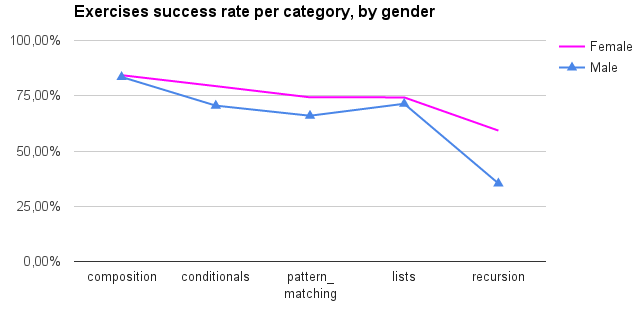
\includegraphics[width=0.4\textwidth]{graphics/success-rate-per-category-by-gender.png}
%    \caption{Caption}
%    \label{fig:success-rate-by-gender}
%\end{figure}

%classify the findings according to some criteria %1 page (everybody), results

\section{Previous work and dicussion} \label{previous-work}

%length: 1 page
%resposible: Lu & Gui

%content:
%previous work on Smart Content for CS education and automatic formative feedback

In this section we discuss our results and we briefly review previous work on educative coding tools to teach functional programming. 

As we mentioned in Section~\ref{introduction}, almost all educative coding tools focus on imperative or object oriented programming languages. Moreover, most of these tools are generally only used in a single  university, usually when they were developed~\cite{brusilovsky2014increasing}. To the best of our knowledge, there is only one coding tool for Haskell that was developed with educative purposes: Ask-Elle.  

% WIP (Guillaume)
%Let us review previous Smart Learning Content~\cite{brusilovsky2014increasing} for
%functional programming teaching, with automatic formative feedback: Ask-Elle for Haskell and Programmer's Learning Machine for Scala.

Ask-Elle~\cite{Gerdes:2012,gerdes2016ask} is a web-based tutor
that shares many features with Mumuki. It provides exercises in Haskell with automatic feedback. As with Mumuki, each exercise is automatically evaluated using tests and strategies, the latter
being similar to Mumuki's expectations. Strategies use syntactical analysis but also program
transformation to drive automatic feedback, that is, tests and hints.
As for tests, Ask-Elle uses QuickCheck~\cite{Claessen2000} to generate random tests in order to evaluate for correctness. This
impedes some students' strategy of making programs pass only for a finite number of tests,
as is possible for some of Mumuki's exercises.
%Finally, Ask-Elle does not provide the console feature of Mumuki.

Ask-Elle was evaluated in several experiments at a single University. The students performance on the exercises  automatically evaluated by the tool was reported but it was not analysed by topic nor comparatively between students with different backgrounds. The students attitude towards the tool was evaluated through a questionnaire as we did. However, the authors do not report following any standard methodology. Its effect on course dropouts was not reported but the authors report that the students considered Ask-Elle feedback useful when they found difficult exercises.  

Differently from Mumuki, Ask-Elle allows a teacher to specify different correct solutions for each exercise and to predict common errors and provide appropriate feedback when designing an exercise. Given our results when applying TAM, we believe that Mumuki could also benefit from improved feedback. However, the method implemented in Ask-Elle is too time consuming for teachers so we plan to improve the feedback using data-driven techniques that mine previous students solutions and previous teacher feedback~\cite{Price:2015}. In our study , we observed that feedback was assessed as better in the CS1 course compared to the CS3 course. This may be due to the fact that the CS1 course included a second stage where common errors were explained by the teacher and students were encouraged to manually test their code on paper. We plan to further investigate this in future work.  

We found a few educative coding tools for another functional language, namely Scala. A representative example is the Programmer's Learning Machine. 
The Programmer's Learning Machine~\cite{quinson2015teaching} (PLM) is a client-side program
that provides several kinds of microworlds, in which student's programs are visualized
when executed. It provides series of exercices that can be solved with the imperative
languages Java and Python, as with the funcional language Scala.
As most of the microworlds in PLM are graphical, the
feedback provided is purely visual, which is not comparable with the feedback Mumuki provides. One exception is the
microworld ``Unit Testing'', which provides test-based feedback. PLM does not provide
feedback based on syntactical analysis nor program transformations. %1 page (Lu & Gui), CS smart content 


\section{Conclusions} \label{conclusion}

%length: 1 page including references and acks
%resposible: everybody

%content:

Through two university interventions focusing on learning a functional programming language with the assistance of an online coding tool we found that students benefit from the availability of such tool and that they assess it positively. In spite of these results and previous work, the adoption of these tools is not widespread and they are usually used only in the university where they were created (as discussed in~\cite{brusilovsky2014increasing}). We present in this paper two interventions in two different universities where the teachers adopt the tool in spite of not being the developers.
CS1 students seem to benefit more from using Mumuki than CS3 students. Their dropout rate was improved more than in CS3 and their assess the usefulness of the tool more positively although it was harder for them to complete the exercises. Differently from previous work we found no gender differences neither in performance nor in attitude. 
 
There are several implication of our findings. 1) Based on our research and on previous work we suggest that student dropout rate may diminish when using educative coding tools when learning to program. In our study this is particularly so in CS1. 2) Students can transfer programming skills from imperative languages into functional languages but they also can learn functional languages as their first programming language without difficulties. 3) The logs of these online tools can serve to explore the most common errors and explain them in-class. Thorough in-class explanations diminishes the need of better automated feedback but are time consuming. We will explore the automatic generation of better feedback on errors with data-driven methods in future work. 

%After finishing this course our students continued using Mumuki to learn other programming languages on their own and 95\% said that they wanted to continue using it in the future.  

 
 %1 page (everybody) including references

%\section*{Acknowledgments}
%\vspace*{-.4cm}
%This work was partially funded by grants PICT-2014-1833, PDTS-CIN-CONICET-2015-172, and PID-2012-2013-R18. 


%\end{document}  % This is where a 'short' article might terminate

%ACKNOWLEDGMENTS are optional
%
% The following two commands are all you need in the
% initial runs of your .tex file to
% produce the bibliography for the citations in your paper.
\bibliographystyle{abbrv}
\bibliography{sigproc}  % sigproc.bib is the name of the Bibliography in this case
% You must have a proper ".bib" file
%  and remember to run:
% latex bibtex latex latex
% to resolve all references
%
% ACM needs 'a single self-contained file'!
%
%APPENDICES are optional
%\balancecolumns

\end{document}
